\section{Categorization}
Categorization is the process of grouping collections of text into categories, and can be done by both humans or computers. Computer categorization is the technique of teaching a classifier how to decide the category of any input \cite{wiki:categorization}. The idea of this process is to find patterns which makes the machine able to predict the category or class of the input. Such patterns could be similarities between input or decision rules \cite{wiki:classification}. It is desirable to optimize the results of the classifier so that the classifier is as accurate as possible. This can be done by learning the classifier how to behave, either by machine learning where the classifier optimizes itself based on feedback, or by improving the classifier's decision rules.  \\\\
%make the classifier as good as possible,
%Categorization with machine learning can be split into further types; statistical classification which is a \emph{supervised} learning process, and clustering which can be performed as both %an \textit{supervised} and a \emph{supervised} and an \emph{unsupervised} learning process. Supervised learning is a technique where the machine is given a training data set, where the set contains the correct output in addition to the input we want to classify. The classifier uses this data to learn the machine how to behave, also called training the classifier. Unsupervised learning, on the other hand, is the task of trying to find a hidden structure in unlabeled data. The main difference between the two types is that unlabeled data gives no feedback to the classifier, hence the classifier has to assume that it is correctly classified without receiving feedback. It is also possible to have classification processes which are combined of the two, where prior knowledge is given to the classifier. 
%added to the classification process for better results. 
%the data is unlabeled is no feedback sent to the classifier. 
%The classifier will therefore not know if the result is correct, but will continue to classify assuming that the classification performed so far is correct.  
Our problem consists of two categorization problems: 
\begin{enumerate}
\item Categorization of keywords.
\item Categorization of any text.
\end{enumerate}

%the main categorization where any article given as input should be categorized to its most describing category.  

\subsubsection{Categorization of keywords}
The categorization of keywords is done by creating a keyword list based on titles of Wikipedia articles. These keywords have to be categorized to suitable output categories. This categorization could be split into two parts: 

\begin{enumerate}
\item Categorize the keywords to Wikipedia categories represented as category paths  (see figure \ref{fig:keywords_to_categories}). This categorization should be based on the content of the Wikipedia articles of the keywords. Our assumption is that the meaning of a Wikipedia article can be found by looking at the underlying structure of Wikipedia, i.e., the article's categories and the category structure.\begin{figure}[h]
\centering
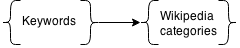
\includegraphics[width=0.4\textwidth]{Chapters/Background/Keywords_to_categories}
\caption[Categorization of keywords to Wikipedia categories]{Illustration of the categorization of keywords to Wikipedia categories.}
\label{fig:keywords_to_categories}
\end{figure}
\item The complete categorization of the keywords are based on creating a connection between the keywords and categories from IAB's taxonomy (see figure \ref{fig:keywords_categorization_full}). This categorization is based on rules between excerpts of Wikipedia category paths and the output categories. 
\begin{figure}[h]
\centering
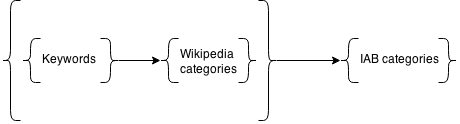
\includegraphics[width=0.7\textwidth]{Chapters/Background/Keywords_categorization_full}
\caption[Categorzation process of the keywords]{Illustration of the complete categorization process of the keywords.}
\label{fig:keywords_categorization_full}
\end{figure}
\end{enumerate}
%the categorization by finding rules and apply heuristics. 

%The categorization needed to determine the categories for each article is a statistical classification. Wikipedia's structure is available and this can be used to find the most likely categories. 

\subsubsection{Categorization of any text}
The goal for this project is to be able to categorize any text based on the results from the categorization of the keywords. The classifier for this categorization process needs some rules on how it should classify. Our theory is that occurrences of keywords can determine the content of the text, and multiple keywords categorized to the same category indicate that the text should be categorized to this category. Thus, the classifier needs a way of detecting keywords in the text and a way of determining which category the text belongs to if it contains keywords from different categories. 


%. The main assumption 

%The next classification problem is to classify 
%Our main assumption for content analysis is that articles which contains the same keywords also belong to some of the same categories in Wikipedia. This means that we want create a group of these articles so that similar articles are grouped together. Supervised classification requires, as already mentioned, a training set. The training set of our problem can be defined as articles in Wikipedia since they are already connected to a category within Wikipedia. The task is to create the classifier that use  this information and is able to classify all other articles. 

%does not have a training set because it is almost impossible to create a training set representiing such a large data set. We still have, however,  information about the underlying category structure of the articles in Wikipedia. The goal is therefore to use this information to group similar articles together.
%Our problem is not suitable for supervised machine learning. Trying to solve the problem with supervised classification would lead to some problems that are difficult to solve; it is for instance almost impossible to create a training set to represent such a large data set and it is therefore not possible to create a classification model based on the data. The categorization should therefore be done with unsupervised machine learning, for instance clustering.

%The formal definition of cluster analysis or clustering is the task of grouping similar elements together.Hence the group or cluster should contain elements that share similarities or that are more similar to each other than to the rest of the elements. %This means that elements within a group are more similar to each other than to the rest of the elements, or that the elements within the group have some similarities that make them stand out from the others. 
%Our problem could therefore be defined as a clustering problem, where each cluster or group is the articles which contains some of the same keywords. We want to sort the texts in such a way that texts with similar content are classified to the same cluster and therefore to same category. The problem needs a mapping process so that collections of texts get clustered together within the predefined set of categories. The predefined set of categories will change depending on the purpose of the classification, for instance would advertisement need a different set of categories than categorization of news articles. A proposal to a predefined category set for advertisement is the category set of IAB. 